% AXI Protocol Presentation - Beamer
\documentclass[aspectratio=169]{beamer}

% Theme and colors
\usetheme{default}
\usecolortheme{default}

% Packages
\usepackage{tikz}
\usepackage{graphicx}
\usepackage{booktabs}
\usepackage{array}
\usepackage{multirow}

% TikZ libraries
\usetikzlibrary{arrows.meta,shapes,positioning,calc,backgrounds,fit}

% Color scheme (Midnight Executive - clean tech look)
\definecolor{primaryblue}{HTML}{1E2761}
\definecolor{lightblue}{HTML}{CADCFC}
\definecolor{accentwhite}{HTML}{FFFFFF}

% Beamer colors
\setbeamercolor{structure}{fg=primaryblue}
\setbeamercolor{frametitle}{bg=primaryblue,fg=accentwhite}
\setbeamercolor{title}{bg=primaryblue,fg=accentwhite}

% Header with logo
\setbeamertemplate{headline}{
  \begin{beamercolorbox}[wd=\paperwidth,ht=11.5ex,dp=1.5ex]{}
    \hfill
    \includegraphics[height=1cm]{images/chips_logo.png}
    \hspace{0.3cm}
  \end{beamercolorbox}
}

% Footer with page numbers
\setbeamertemplate{footline}{
  \hfill
  \insertframenumber{} / \inserttotalframenumber
  \hspace{0.3cm}
  \vspace{0.3cm}
}

% Remove navigation symbols
\setbeamertemplate{navigation symbols}{}

% Title information
\title{Introduction to AXI Protocol}
\subtitle{For High-Performance Memory Controllers}
\date{}

\begin{document}

% ==================== SLIDE 1: Title ====================
\begin{frame}
  \titlepage
\end{frame}

% ==================== SLIDE 2: What is AXI? ====================
\begin{frame}{What is AXI?}
  \begin{columns}
    \begin{column}{0.55\textwidth}
      \textbf{AMBA Advanced eXtensible Interface}
      
      \vspace{0.5cm}
      
      \textbf{Design Goals:}
      \begin{itemize}
        \item High bandwidth, low latency
        \item High-frequency operation
        \item Flexible (wide range of components)
        \item \textcolor{primaryblue}{\textbf{Optimized for memory controllers}} with high initial access latency
      \end{itemize}
      
      \vspace{0.5cm}
      
      \textbf{Key Innovation:}\\
      Burst-based transactions with out-of-order completion
    \end{column}
    
    \begin{column}{0.4\textwidth}
      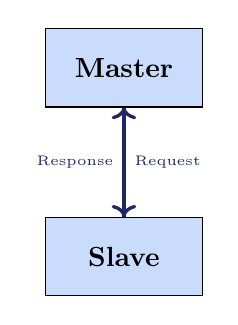
\begin{tikzpicture}[scale=0.8]
        % Master
        \node[rectangle, draw, fill=lightblue, minimum width=2cm, minimum height=1cm] (master) at (0,3) {\textbf{Master}};
        
        % Slave
        \node[rectangle, draw, fill=lightblue, minimum width=2cm, minimum height=1cm] (slave) at (0,0) {\textbf{Slave}};
        
        % Arrows
        \draw[->, very thick, primaryblue] (master.south) -- node[right] {\tiny Request} (slave.north);
        \draw[->, very thick, primaryblue] (slave.north) -- node[left] {\tiny Response} (master.south);
        
      \end{tikzpicture}
      
      \vspace{0.3cm}
      \centering
      \small Perfect for DDR Memory!
    \end{column}
  \end{columns}
\end{frame}

% ==================== SLIDE 3: AXI Versions ====================
\begin{frame}{AXI Protocol Versions}
  \begin{table}
    \centering
    \begin{tabular}{lccc}
      \toprule
      \textbf{Feature} & \textbf{AXI3} & \textbf{AXI4} & \textbf{AXI4-Lite} \\
      \midrule
      Burst Length & 1-16 beats & \textcolor{primaryblue}{\textbf{1-256 beats}} & 1 beat only \\
      Write Interleaving & Yes (WID) & \textcolor{primaryblue}{\textbf{No (removed)}} & N/A \\
      QoS Signaling & No & \textcolor{primaryblue}{\textbf{Yes}} & No \\
      Region Signals & No & Yes & No \\
      Use Case & Legacy & \textbf{Memory Ctrl} & Simple Periph \\
      \bottomrule
    \end{tabular}
  \end{table}
  
  \vspace{0.5cm}
  
  \begin{center}
    \colorbox{lightblue}{\textbf{AXI4 recommended for new memory controller designs}}
  \end{center}
\end{frame}

% ==================== SLIDE 4: Five Channel Architecture ====================
\begin{frame}{Five Independent Channels}
  \begin{center}
    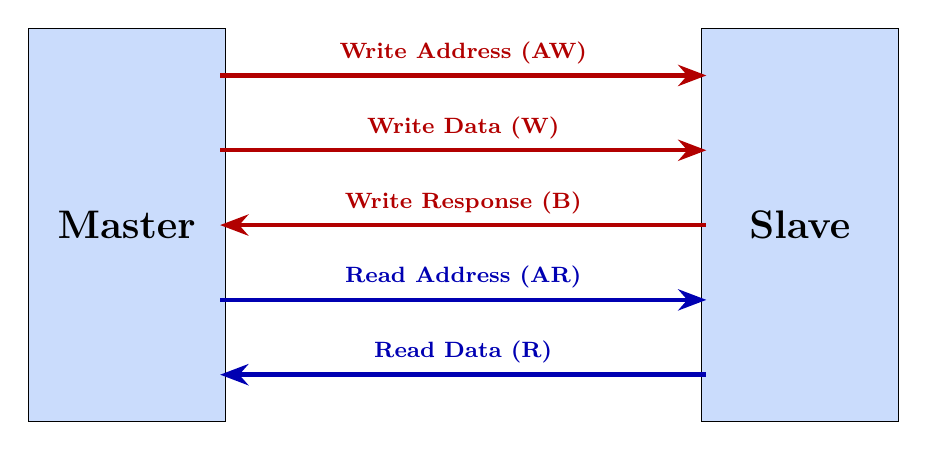
\begin{tikzpicture}[>=Stealth, scale=0.95]
      % Master
      \node[rectangle, draw, fill=lightblue, minimum width=2.5cm, minimum height=5cm, font=\Large\bfseries] (master) at (0,0) {Master};
      
      % Slave
      \node[rectangle, draw, fill=lightblue, minimum width=2.5cm, minimum height=5cm, font=\Large\bfseries] (slave) at (9,0) {Slave};
      
      % Write channels (top to bottom, better spacing)
      \draw[->, ultra thick, red!70!black] (1.25,2) -- node[above, font=\footnotesize] {\textbf{Write Address (AW)}} (7.75,2);
      \draw[->, ultra thick, red!70!black] (1.25,1) -- node[above, font=\footnotesize] {\textbf{Write Data (W)}} (7.75,1);
      \draw[<-, ultra thick, red!70!black] (1.25,0) -- node[above, font=\footnotesize] {\textbf{Write Response (B)}} (7.75,0);
      
      % Read channels (bottom)
      \draw[->, ultra thick, blue!70!black] (1.25,-1) -- node[above, font=\footnotesize] {\textbf{Read Address (AR)}} (7.75,-1);
      \draw[<-, ultra thick, blue!70!black] (1.25,-2) -- node[above, font=\footnotesize] {\textbf{Read Data (R)}} (7.75,-2);
      
    \end{tikzpicture}
  \end{center}
  
  \vspace{0.3cm}
  
  \begin{center}
    \textbf{Key Benefit:} Read and Write operate \textcolor{primaryblue}{\textbf{simultaneously}} (full duplex)
  \end{center}
\end{frame}

% ==================== SLIDE 5: Write Transaction Channels ====================
\begin{frame}{Write Transaction Channels}
  \begin{columns}
    \begin{column}{0.45\textwidth}
      \textbf{Write Address (AW)}
      \begin{itemize}
        \item AWID, AWADDR
        \item AWLEN, AWSIZE
        \item AWBURST, AWQOS
      \end{itemize}
      
      \vspace{0.5cm}
      
      \textbf{Write Data (W)}
      \begin{itemize}
        \item WDATA, WSTRB
        \item WLAST
      \end{itemize}
      
      \vspace{0.5cm}
      
      \textbf{Write Response (B)}
      \begin{itemize}
        \item BID, BRESP
      \end{itemize}
    \end{column}
    
    \begin{column}{0.5\textwidth}
      \centering
      \includegraphics[width=\textwidth]{images/axi_channel_write.png}
    \end{column}
  \end{columns}
\end{frame}

% ==================== SLIDE 6: Read Transaction Channels ====================
\begin{frame}{Read Transaction Channels}
  \begin{columns}
    \begin{column}{0.48\textwidth}
      \textbf{1. Read Address (AR)}
      \begin{itemize}
        \item ARID - Transaction ID
        \item ARADDR - Start address
        \item ARLEN - Burst length
        \item ARSIZE - Bytes per beat
        \item ARBURST - Type (FIXED/INCR/WRAP)
        \item ARQOS - Priority (AXI4)
      \end{itemize}
    \end{column}
    
    \begin{column}{0.48\textwidth}
      \textbf{2. Read Data (R)}
      \begin{itemize}
        \item RID - Matches ARID
        \item RDATA - Actual data
        \item RRESP - Status
        \item RLAST - Final beat indicator
      \end{itemize}
    \end{column}
  \end{columns}
\end{frame}

% ==================== SLIDE 7: Read Channel Diagram ====================
\begin{frame}{Read Channel Diagram}
  \begin{center}
    \includegraphics[width=0.85\textwidth]{images/axi_channel_read.png}
  \end{center}
\end{frame}

% ==================== SLIDE 7: VALID/READY Handshake ====================
\begin{frame}{VALID/READY Handshake Protocol}
  \begin{columns}
    \begin{column}{0.45\textwidth}
      \textbf{Every channel uses:}
      \begin{itemize}
        \item \textbf{VALID} - Source has data
        \item \textbf{READY} - Destination can accept
        \item \textbf{Transfer} - Both HIGH
      \end{itemize}
      
      \vspace{0.5cm}
      
      \textbf{Critical Rules:}
      \begin{itemize}
        \item VALID \textcolor{red}{\textbf{must NOT}} wait for READY
        \item READY \textcolor{primaryblue}{\textbf{can}} wait for VALID
        \item Prevents deadlock!
      \end{itemize}
    \end{column}
    
    \begin{column}{0.5\textwidth}
      \centering
      \includegraphics[width=\textwidth]{images/valid_with_ready.png}
      
      \vspace{0.3cm}
      
      \includegraphics[width=\textwidth]{images/ready_b4_valid.png}
    \end{column}
  \end{columns}
\end{frame}

% ==================== SLIDE 8: Burst Parameters ====================
\begin{frame}{Burst Transaction Parameters}
  \begin{table}
    \centering
    \begin{tabular}{lll}
      \toprule
      \textbf{Parameter} & \textbf{Encoding} & \textbf{Meaning} \\
      \midrule
      AWLEN/ARLEN & 0-255 (AXI4) & Beats = LEN + 1 \\
      & 0-15 (AXI3) & \\
      \midrule
      AWSIZE/ARSIZE & 3 bits & Bytes/beat = $2^{SIZE}$ \\
      & 000 $\rightarrow$ 1 byte & \\
      & 011 $\rightarrow$ 8 bytes & \\
      & 111 $\rightarrow$ 128 bytes & \\
      \bottomrule
    \end{tabular}
  \end{table}
  
  \vspace{0.5cm}
  
  \begin{center}
    \colorbox{lightblue}{
      \parbox{0.8\textwidth}{
        \centering
        \textbf{Total Burst Size} = (AWLEN + 1) × $2^{AWSIZE}$ \\
        \vspace{0.2cm}
        \textbf{AXI4 Max:} 256 beats × 128 bytes = \textcolor{primaryblue}{\textbf{32 KB}} per burst!
      }
    }
  \end{center}
\end{frame}

% ==================== SLIDE 9: Burst Types ====================
\begin{frame}{Burst Types}
  \vspace{0.3cm}
  \begin{center}
    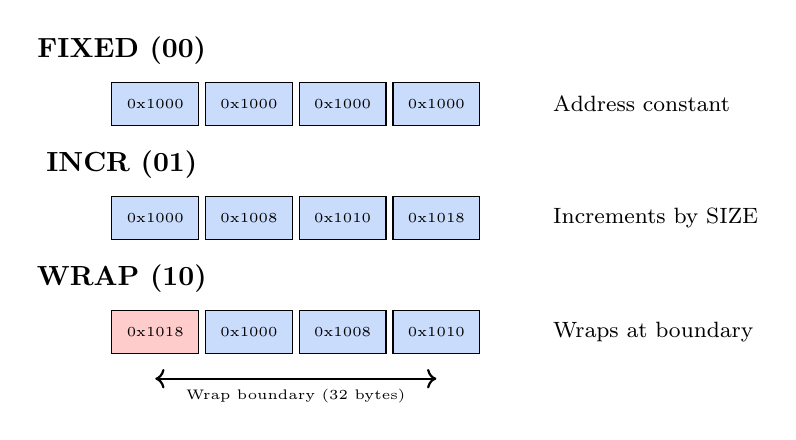
\begin{tikzpicture}[scale=0.85, every node/.style={font=\small}]
      % FIXED
      \node[font=\bfseries] at (-0.5,3.8) {FIXED (00)};
      \foreach \x in {0,1,2,3} {
        \node[rectangle, draw, fill=lightblue, minimum width=1.1cm, minimum height=0.55cm] at (\x*1.4, 3) {\tiny 0x1000};
      }
      \node[right, font=\footnotesize] at (5.8,3) {Address constant};
      
      % INCR
      \node[font=\bfseries] at (-0.5,2.1) {INCR (01)};
      \node[rectangle, draw, fill=lightblue, minimum width=1.1cm, minimum height=0.55cm] at (0, 1.3) {\tiny 0x1000};
      \node[rectangle, draw, fill=lightblue, minimum width=1.1cm, minimum height=0.55cm] at (1.4, 1.3) {\tiny 0x1008};
      \node[rectangle, draw, fill=lightblue, minimum width=1.1cm, minimum height=0.55cm] at (2.8, 1.3) {\tiny 0x1010};
      \node[rectangle, draw, fill=lightblue, minimum width=1.1cm, minimum height=0.55cm] at (4.2, 1.3) {\tiny 0x1018};
      \node[right, font=\footnotesize] at (5.8,1.3) {Increments by SIZE};
      
      % WRAP
      \node[font=\bfseries] at (-0.5,0.4) {WRAP (10)};
      \node[rectangle, draw, fill=red!20, minimum width=1.1cm, minimum height=0.55cm] at (0, -0.4) {\tiny 0x1018};
      \node[rectangle, draw, fill=lightblue, minimum width=1.1cm, minimum height=0.55cm] at (1.4, -0.4) {\tiny 0x1000};
      \node[rectangle, draw, fill=lightblue, minimum width=1.1cm, minimum height=0.55cm] at (2.8, -0.4) {\tiny 0x1008};
      \node[rectangle, draw, fill=lightblue, minimum width=1.1cm, minimum height=0.55cm] at (4.2, -0.4) {\tiny 0x1010};
      \node[right, font=\footnotesize] at (5.8,-0.4) {Wraps at boundary};
      
      \draw[<->, thick] (0,-1.1) -- node[below, font=\tiny] {Wrap boundary (32 bytes)} (4.2,-1.1);
    \end{tikzpicture}
  \end{center}
  
  \vspace{0.3cm}
  
  \begin{center}
    \small \textbf{Most common for DDR:} INCR \hspace{1cm} \textbf{For caches:} WRAP
  \end{center}
\end{frame}

% ==================== SLIDE 10: Write Burst ====================
\begin{frame}{Write Burst Example}
  \begin{center}
    \includegraphics[width=0.9\textwidth]{images/axi_write_burst.png}
  \end{center}
  
  \vspace{0.3cm}
  
  \begin{center}
    \textbf{Note:} Address sent once, multiple data beats follow
  \end{center}
\end{frame}

% ==================== SLIDE 11: Read Burst ====================
\begin{frame}{Read Burst Example}
  \begin{center}
    \includegraphics[width=0.9\textwidth]{images/axi_read_burst.png}
  \end{center}
  
  \vspace{0.3cm}
  
  \begin{center}
    \textbf{Slave returns multiple data beats} for single address request
  \end{center}
\end{frame}

% ==================== SLIDE 12: Overlapping Bursts ====================
\begin{frame}{Overlapping Bursts (Pipelining)}
  \begin{center}
    \includegraphics[width=0.9\textwidth]{images/axi_overlapping_read_burst.png}
  \end{center}
  
  \vspace{0.3cm}
  
  \begin{center}
    \textbf{Multiple transactions in flight} $\rightarrow$ Hides memory latency!
  \end{center}
\end{frame}

% ==================== SLIDE 14: Transaction IDs ====================
\begin{frame}{Transaction IDs \& Out-of-Order Completion}
  \begin{columns}
    \begin{column}{0.48\textwidth}
      \textbf{Why IDs?}
      \begin{itemize}
        \item Memory has high latency
        \item Issue multiple requests
        \item Complete when ready
        \item Use ID to route response
      \end{itemize}
      
      \vspace{0.5cm}
      
      \textbf{Ordering Rules:}
      \begin{itemize}
        \item \textcolor{primaryblue}{\textbf{Same ID}} $\rightarrow$ In-order
        \item \textcolor{red}{\textbf{Different ID}} $\rightarrow$ Any order
      \end{itemize}
    \end{column}
    
    \begin{column}{0.48\textwidth}
      \centering
      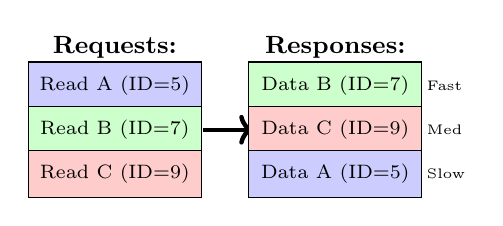
\begin{tikzpicture}[scale=0.8]
        % Requests box
        \node[font=\small\bfseries] at (0,3.3) {Requests:};
        \node[rectangle, draw, fill=blue!20, font=\scriptsize, minimum width=2.2cm, minimum height=0.6cm] (r1) at (0,2.7) {Read A (ID=5)};
        \node[rectangle, draw, fill=green!20, font=\scriptsize, minimum width=2.2cm, minimum height=0.6cm] (r2) at (0,2.0) {Read B (ID=7)};
        \node[rectangle, draw, fill=red!20, font=\scriptsize, minimum width=2.2cm, minimum height=0.6cm] (r3) at (0,1.3) {Read C (ID=9)};
        
        % Arrow
        \draw[->, ultra thick] (1.4,2.0) -- (2.2,2.0);
        
        % Responses box
        \node[font=\small\bfseries] at (3.5,3.3) {Responses:};
        \node[rectangle, draw, fill=green!20, font=\scriptsize, minimum width=2.2cm, minimum height=0.6cm] (s2) at (3.5,2.7) {Data B (ID=7)};
        \node[right, font=\tiny] at (4.8,2.7) {Fast};
        \node[rectangle, draw, fill=red!20, font=\scriptsize, minimum width=2.2cm, minimum height=0.6cm] (s3) at (3.5,2.0) {Data C (ID=9)};
        \node[right, font=\tiny] at (4.8,2.0) {Med};
        \node[rectangle, draw, fill=blue!20, font=\scriptsize, minimum width=2.2cm, minimum height=0.6cm] (s1) at (3.5,1.3) {Data A (ID=5)};
        \node[right, font=\tiny] at (4.8,1.3) {Slow};
      \end{tikzpicture}
      
      \vspace{0.3cm}
      \small Out-of-order = Performance!
    \end{column}
  \end{columns}
\end{frame}

% ==================== SLIDE 14: AXI4 Enhancements ====================
\begin{frame}{AXI4 Enhancements Over AXI3}
  \begin{columns}
    \begin{column}{0.48\textwidth}
      \textbf{Performance:}
      \begin{itemize}
        \item \textcolor{primaryblue}{\textbf{256 beat bursts}} (was 16)
        \item Longer sequential access
        \item Better DDR utilization
      \end{itemize}
      
      \vspace{0.5cm}
      
      \textbf{Quality of Service:}
      \begin{itemize}
        \item ARQOS/AWQOS signals
        \item 4-bit priority (0-15)
        \item Real-time traffic prioritization
      \end{itemize}
    \end{column}
    
    \begin{column}{0.48\textwidth}
      \textbf{Simplification:}
      \begin{itemize}
        \item \textcolor{red}{\textbf{Removed WID}} signal
        \item No write data interleaving
        \item Simpler slave implementation
        \item Less hardware complexity
      \end{itemize}
      
      \vspace{0.5cm}
      
      \textbf{Additional:}
      \begin{itemize}
        \item Region identifiers
        \item User-defined signals
        \item Enhanced cache attributes
      \end{itemize}
    \end{column}
  \end{columns}
\end{frame}

% ==================== SLIDE 15: AXI to DDR Translation ====================
\begin{frame}{AXI to DDR Command Translation}
  \begin{columns}
    \begin{column}{0.48\textwidth}
      \textbf{AXI Read Request:}
      \begin{itemize}
        \item ARADDR = 0x9000\_1000
        \item ARLEN = 7 (8 beats)
        \item ARSIZE = 3 (8 bytes)
      \end{itemize}
      
      \vspace{0.5cm}
      
      \textbf{Memory Controller Decodes:}
      \begin{itemize}
        \item Bank = 2
        \item Row = 0x900
        \item Column = 0x10
      \end{itemize}
    \end{column}
    
    \begin{column}{0.48\textwidth}
      \textbf{DDR Commands Issued:}

      \vspace{0.35cm}

      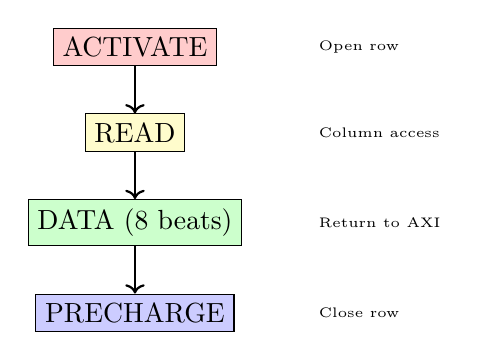
\begin{tikzpicture}[node distance=0.6cm]
        \node[rectangle, draw, fill=red!20] (act) {ACTIVATE};
        \node[below=of act, rectangle, draw, fill=yellow!20] (read) {READ};
        \node[below=of read, rectangle, draw, fill=green!20] (data) {DATA (8 beats)};
        \node[below=of data, rectangle, draw, fill=blue!20] (pre) {PRECHARGE};

        \draw[->, thick] (act) -- (read);
        \draw[->, thick] (read) -- (data);
        \draw[->, thick] (data) -- (pre);

        % compute a single x-position for the label column (use the widest box as baseline)
        \coordinate (labelx) at ($(data.east)+(0.85cm,0)$);
        \node[anchor=west, font=\tiny] at (labelx |- act) {Open row};
        \node[anchor=west, font=\tiny] at (labelx |- read) {Column access};
        \node[anchor=west, font=\tiny] at (labelx |- data) {Return to AXI};
        \node[anchor=west, font=\tiny] at (labelx |- pre) {Close row};
      \end{tikzpicture}
    \end{column}
  \end{columns}
\end{frame}

% ==================== SLIDE 16: Why AXI for DDR ====================
\begin{frame}{Why AXI is Perfect for DDR Memory Controllers}
  \begin{center}
    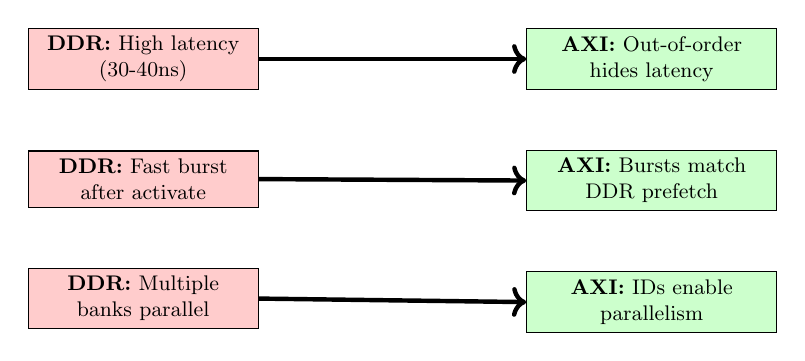
\begin{tikzpicture}[node distance=0.9cm, scale=0.85, every node/.style={transform shape}]
      % DDR challenges
      \node[rectangle, draw, fill=red!20, text width=3.2cm, align=center, font=\small] (lat) {\textbf{DDR:} High latency\\(30-40ns)};
      \node[below=of lat, rectangle, draw, fill=red!20, text width=3.2cm, align=center, font=\small] (burst) {\textbf{DDR:} Fast burst\\after activate};
      \node[below=of burst, rectangle, draw, fill=red!20, text width=3.2cm, align=center, font=\small] (bank) {\textbf{DDR:} Multiple\\banks parallel};
      
      % AXI solutions
      \node[right=4cm of lat, rectangle, draw, fill=green!20, text width=3.5cm, align=center, font=\small] (sol1) {\textbf{AXI:} Out-of-order\\hides latency};
      \node[below=of sol1, rectangle, draw, fill=green!20, text width=3.5cm, align=center, font=\small] (sol2) {\textbf{AXI:} Bursts match\\DDR prefetch};
      \node[below=of sol2, rectangle, draw, fill=green!20, text width=3.5cm, align=center, font=\small] (sol3) {\textbf{AXI:} IDs enable\\parallelism};
      
      % Arrows connecting each pair
      \draw[->, ultra thick] (lat.east) -- (sol1.west);
      \draw[->, ultra thick] (burst.east) -- (sol2.west);
      \draw[->, ultra thick] (bank.east) -- (sol3.west);
    \end{tikzpicture}
  \end{center}
  
  \vspace{0.5cm}
  
  \begin{center}
    \colorbox{lightblue}{\textbf{Perfect match between protocol and memory!}}
  \end{center}
\end{frame}

% ==================== SLIDE 18: Memory Controller Optimizations ====================
\begin{frame}{Memory Controller Optimizations Using AXI}
  \begin{columns}
    \begin{column}{0.48\textwidth}
      \textbf{Transaction Reordering:}
      \begin{itemize}
        \item Row buffer hits first
        \item Bank parallelism
        \item Min read/write switch
      \end{itemize}
      
      \vspace{0.8cm}
      
      \textbf{QoS Scheduling:}
      \begin{itemize}
        \item Priority-based (ARQOS/AWQOS)
        \item Real-time = high priority
        \item DMA = low priority
      \end{itemize}
    \end{column}
    
    \begin{column}{0.48\textwidth}
      \textbf{Write Buffering:}
      \begin{itemize}
        \item Collect small writes
        \item Combine to DDR bursts
        \item Early response (BRESP)
      \end{itemize}
      
      \vspace{0.8cm}
      
      \textbf{Burst Alignment:}
      \begin{itemize}
        \item Match DDR BL8
        \item Align to cache lines
        \item Respect 4KB boundary
      \end{itemize}
    \end{column}
  \end{columns}
\end{frame}

% ==================== SLIDE 19: Key Takeaways ====================
\begin{frame}{Key Takeaways}
  \begin{center}
    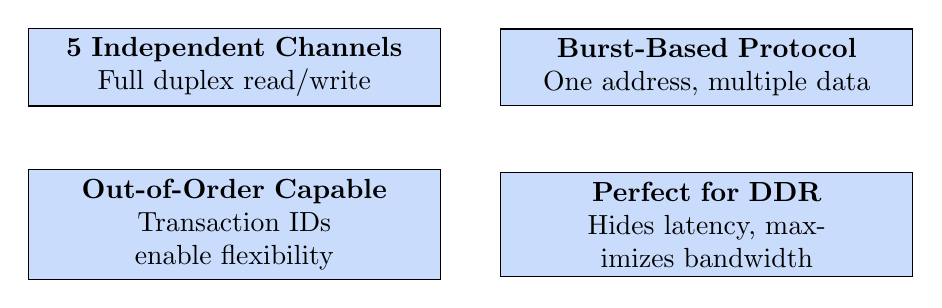
\begin{tikzpicture}
      % Key points in boxes
      \node[rectangle, draw, fill=lightblue, text width=5cm, align=center] (c1) at (0,2) {
        \textbf{5 Independent Channels}\\
        Full duplex read/write
      };
      
      \node[rectangle, draw, fill=lightblue, text width=5cm, align=center] (c2) at (6,2) {
        \textbf{Burst-Based Protocol}\\
        One address, multiple data
      };
      
      \node[rectangle, draw, fill=lightblue, text width=5cm, align=center] (c3) at (0,0) {
        \textbf{Out-of-Order Capable}\\
        Transaction IDs enable flexibility
      };
      
      \node[rectangle, draw, fill=lightblue, text width=5cm, align=center] (c4) at (6,0) {
        \textbf{Perfect for DDR}\\
        Hides latency, maximizes bandwidth
      };
    \end{tikzpicture}
  \end{center}
  
  \vspace{0.8cm}
  
  \begin{center}
    \textbf{Critical Rules:}\\
    \small
    VALID must NOT wait for READY $\bullet$ 
    Bursts cannot cross 4KB $\bullet$
    Same ID = ordered
  \end{center}
\end{frame}

\end{document}